% Options for packages loaded elsewhere
\PassOptionsToPackage{unicode}{hyperref}
\PassOptionsToPackage{hyphens}{url}
%
\documentclass[
]{article}
\usepackage{amsmath,amssymb}
\usepackage{lmodern}
\usepackage{iftex}
\ifPDFTeX
  \usepackage[T1]{fontenc}
  \usepackage[utf8]{inputenc}
  \usepackage{textcomp} % provide euro and other symbols
\else % if luatex or xetex
  \usepackage{unicode-math}
  \defaultfontfeatures{Scale=MatchLowercase}
  \defaultfontfeatures[\rmfamily]{Ligatures=TeX,Scale=1}
\fi
% Use upquote if available, for straight quotes in verbatim environments
\IfFileExists{upquote.sty}{\usepackage{upquote}}{}
\IfFileExists{microtype.sty}{% use microtype if available
  \usepackage[]{microtype}
  \UseMicrotypeSet[protrusion]{basicmath} % disable protrusion for tt fonts
}{}
\makeatletter
\@ifundefined{KOMAClassName}{% if non-KOMA class
  \IfFileExists{parskip.sty}{%
    \usepackage{parskip}
  }{% else
    \setlength{\parindent}{0pt}
    \setlength{\parskip}{6pt plus 2pt minus 1pt}}
}{% if KOMA class
  \KOMAoptions{parskip=half}}
\makeatother
\usepackage{xcolor}
\usepackage[margin=1in]{geometry}
\usepackage{color}
\usepackage{fancyvrb}
\newcommand{\VerbBar}{|}
\newcommand{\VERB}{\Verb[commandchars=\\\{\}]}
\DefineVerbatimEnvironment{Highlighting}{Verbatim}{commandchars=\\\{\}}
% Add ',fontsize=\small' for more characters per line
\usepackage{framed}
\definecolor{shadecolor}{RGB}{248,248,248}
\newenvironment{Shaded}{\begin{snugshade}}{\end{snugshade}}
\newcommand{\AlertTok}[1]{\textcolor[rgb]{0.94,0.16,0.16}{#1}}
\newcommand{\AnnotationTok}[1]{\textcolor[rgb]{0.56,0.35,0.01}{\textbf{\textit{#1}}}}
\newcommand{\AttributeTok}[1]{\textcolor[rgb]{0.77,0.63,0.00}{#1}}
\newcommand{\BaseNTok}[1]{\textcolor[rgb]{0.00,0.00,0.81}{#1}}
\newcommand{\BuiltInTok}[1]{#1}
\newcommand{\CharTok}[1]{\textcolor[rgb]{0.31,0.60,0.02}{#1}}
\newcommand{\CommentTok}[1]{\textcolor[rgb]{0.56,0.35,0.01}{\textit{#1}}}
\newcommand{\CommentVarTok}[1]{\textcolor[rgb]{0.56,0.35,0.01}{\textbf{\textit{#1}}}}
\newcommand{\ConstantTok}[1]{\textcolor[rgb]{0.00,0.00,0.00}{#1}}
\newcommand{\ControlFlowTok}[1]{\textcolor[rgb]{0.13,0.29,0.53}{\textbf{#1}}}
\newcommand{\DataTypeTok}[1]{\textcolor[rgb]{0.13,0.29,0.53}{#1}}
\newcommand{\DecValTok}[1]{\textcolor[rgb]{0.00,0.00,0.81}{#1}}
\newcommand{\DocumentationTok}[1]{\textcolor[rgb]{0.56,0.35,0.01}{\textbf{\textit{#1}}}}
\newcommand{\ErrorTok}[1]{\textcolor[rgb]{0.64,0.00,0.00}{\textbf{#1}}}
\newcommand{\ExtensionTok}[1]{#1}
\newcommand{\FloatTok}[1]{\textcolor[rgb]{0.00,0.00,0.81}{#1}}
\newcommand{\FunctionTok}[1]{\textcolor[rgb]{0.00,0.00,0.00}{#1}}
\newcommand{\ImportTok}[1]{#1}
\newcommand{\InformationTok}[1]{\textcolor[rgb]{0.56,0.35,0.01}{\textbf{\textit{#1}}}}
\newcommand{\KeywordTok}[1]{\textcolor[rgb]{0.13,0.29,0.53}{\textbf{#1}}}
\newcommand{\NormalTok}[1]{#1}
\newcommand{\OperatorTok}[1]{\textcolor[rgb]{0.81,0.36,0.00}{\textbf{#1}}}
\newcommand{\OtherTok}[1]{\textcolor[rgb]{0.56,0.35,0.01}{#1}}
\newcommand{\PreprocessorTok}[1]{\textcolor[rgb]{0.56,0.35,0.01}{\textit{#1}}}
\newcommand{\RegionMarkerTok}[1]{#1}
\newcommand{\SpecialCharTok}[1]{\textcolor[rgb]{0.00,0.00,0.00}{#1}}
\newcommand{\SpecialStringTok}[1]{\textcolor[rgb]{0.31,0.60,0.02}{#1}}
\newcommand{\StringTok}[1]{\textcolor[rgb]{0.31,0.60,0.02}{#1}}
\newcommand{\VariableTok}[1]{\textcolor[rgb]{0.00,0.00,0.00}{#1}}
\newcommand{\VerbatimStringTok}[1]{\textcolor[rgb]{0.31,0.60,0.02}{#1}}
\newcommand{\WarningTok}[1]{\textcolor[rgb]{0.56,0.35,0.01}{\textbf{\textit{#1}}}}
\usepackage{graphicx}
\makeatletter
\def\maxwidth{\ifdim\Gin@nat@width>\linewidth\linewidth\else\Gin@nat@width\fi}
\def\maxheight{\ifdim\Gin@nat@height>\textheight\textheight\else\Gin@nat@height\fi}
\makeatother
% Scale images if necessary, so that they will not overflow the page
% margins by default, and it is still possible to overwrite the defaults
% using explicit options in \includegraphics[width, height, ...]{}
\setkeys{Gin}{width=\maxwidth,height=\maxheight,keepaspectratio}
% Set default figure placement to htbp
\makeatletter
\def\fps@figure{htbp}
\makeatother
\setlength{\emergencystretch}{3em} % prevent overfull lines
\providecommand{\tightlist}{%
  \setlength{\itemsep}{0pt}\setlength{\parskip}{0pt}}
\setcounter{secnumdepth}{-\maxdimen} % remove section numbering
\ifLuaTeX
  \usepackage{selnolig}  % disable illegal ligatures
\fi
\IfFileExists{bookmark.sty}{\usepackage{bookmark}}{\usepackage{hyperref}}
\IfFileExists{xurl.sty}{\usepackage{xurl}}{} % add URL line breaks if available
\urlstyle{same} % disable monospaced font for URLs
\hypersetup{
  pdftitle={Práctica dirigida 5},
  hidelinks,
  pdfcreator={LaTeX via pandoc}}

\title{Práctica dirigida 5}
\author{}
\date{\vspace{-2.5em}}

\begin{document}
\maketitle

{
\setcounter{tocdepth}{2}
\tableofcontents
}
\textbf{FACULTAD DE CIENCIAS SOCIALES - PUCP}

\hypertarget{curso-pol-278---estaduxedstica-para-el-anuxe1lisis-poluxedtico-1-semestre-2025---1}{%
\subsection{\texorpdfstring{Curso: POL 278 - Estadística para el
análisis político 1 \textbar{} Semestre 2025 - 1
}{Curso: POL 278 - Estadística para el análisis político 1 \textbar{} Semestre 2025 - 1  }}\label{curso-pol-278---estaduxedstica-para-el-anuxe1lisis-poluxedtico-1-semestre-2025---1}}

\begin{center}\rule{0.5\linewidth}{0.5pt}\end{center}

\hypertarget{tablas-de-contingencia}{%
\section{\texorpdfstring{\textbf{Tablas de
contingencia}}{Tablas de contingencia}}\label{tablas-de-contingencia}}

\begin{itemize}
\tightlist
\item
  Son tablas de doble entrada, en las cuales se cruzan las categorías de
  dos variables de interés.
\item
  En las casillas de la tabla se ubica la frecuencia o el número de
  casos de cada cruce.
\item
  Conceptos importantes: Frecuencias observadas y frecuencias esperadas.
\end{itemize}

\hypertarget{frecuencias-observadas-y-esperadas}{%
\subsubsection{\texorpdfstring{\textbf{Frecuencias observadas y
esperadas}}{Frecuencias observadas y esperadas}}\label{frecuencias-observadas-y-esperadas}}

\begin{itemize}
\item
  Frecuencia esperada: Estas son las frecuencia que deberían darse si
  las variables fueran independientes.
\item
  Frecuencia observada: Estas son las frecuencias reales que se observa
  en nuestra data.
\end{itemize}

\hypertarget{prueba-chi2}{%
\section{\texorpdfstring{\textbf{Prueba
Chi2}}{Prueba Chi2}}\label{prueba-chi2}}

Chi2 es una prueba para estimar el grado de asociación entre variables
categóricas:

\begin{itemize}
\item
  ``Nominal - Nominal'',
\item
  ``Nominal - Ordinal''
\item
  ``Ordinal - Ordinal''
\end{itemize}

Esto significa que una parte de la variabilidad de una variable puede
ser explicada por otra variable.

\textbf{Supuestos:}

Para analizar asociación se requiere que el número de observaciones
esperadas en cada celda de la tabla de contingencia debe ser
suficientemente grande.

Para fines de este curso, al menos cada celda de la tabla de
contingencia de frecuencias esperadas debe ser de 5.

Ten en cuenta que si estas condiciones no se cumplen, entonces la prueba
podría no funcionar adecuadamente y los resultados de la prueba podrían
no ser válidos.

\textbf{Hipótesis:}

\begin{itemize}
\item
  Hipótesis nula (H0): Las variables son estadísticamente independientes
  (No hay asociación) 🚫
\item
  Hipótesis alternativa (H1): Las variables son estadísticamente
  dependientes (Sí hay asociación)✅
\end{itemize}

\hypertarget{percepciones-sobre-la-situaciuxf3n-del-peruxfa}{%
\section{\texorpdfstring{\textbf{Percepciones sobre la situación del
Perú}}{Percepciones sobre la situación del Perú}}\label{percepciones-sobre-la-situaciuxf3n-del-peruxfa}}

¿Cuál es la percepción de la situación del país a partir de variables
socioeconómicas ? 🤔

Para poder responder a la anterior pregunta se usará la base de datos
del Latin American Public Opinion Project (LAPOP\footnote{\url{https://www.vanderbilt.edu/lapop/ab2023/AB2023-Pulso-de-la-democracia-final-20240219.pdf}})
2023. Este es un estudio de la Universidad de Vanderbilt que realiza
encuestas de opinión pública en 34 países de América, incluyendo Norte,
Centro, Sur y el Caribe. LAPOP mide actitudes, evaluaciones y
experiencias en diversos temas, proporcionando datos comparativos de
alta calidad sobre la democracia, la gobernabilidad y el desarrollo
social en la región.

Cargamos la data:

\begin{Shaded}
\begin{Highlighting}[]
\FunctionTok{library}\NormalTok{(rio)}
\FunctionTok{library}\NormalTok{(dplyr)}
\NormalTok{lapop}\OtherTok{=}\FunctionTok{import}\NormalTok{(}\StringTok{"peru2023.sav"}\NormalTok{)}
\FunctionTok{str}\NormalTok{(lapop)}
\end{Highlighting}
\end{Shaded}

\begin{verbatim}
## 'data.frame':    685 obs. of  11 variables:
##  $ estratopri   : num  1103 1103 1103 1103 1103 ...
##   ..- attr(*, "format.spss")= chr "F8.2"
##  $ ur           : num  1 1 1 1 1 1 1 1 1 1 ...
##   ..- attr(*, "format.spss")= chr "F8.2"
##  $ edad         : num  26 44 68 27 53 43 43 29 57 35 ...
##   ..- attr(*, "format.spss")= chr "F8.2"
##  $ sexo         : num  2 2 1 1 1 1 2 2 2 1 ...
##   ..- attr(*, "format.spss")= chr "F8.2"
##  $ situ_pais    : num  3 3 2 1 3 3 3 3 3 3 ...
##   ..- attr(*, "format.spss")= chr "F8.2"
##  $ situ_personal: num  2 2 3 2 3 3 2 2 3 3 ...
##   ..- attr(*, "format.spss")= chr "F8.2"
##  $ mejor_sistema: num  1 1 2 1 1 2 1 1 2 1 ...
##   ..- attr(*, "format.spss")= chr "F8.2"
##  $ percep_dina  : num  3 2 3 4 3 3 4 3 3 3 ...
##   ..- attr(*, "format.spss")= chr "F8.2"
##  $ calid_esc    : num  3 2 3 3 2 4 2 2 2 2 ...
##   ..- attr(*, "format.spss")= chr "F8.2"
##  $ serv_medic   : num  3 2 3 3 2 4 2 3 2 2 ...
##   ..- attr(*, "format.spss")= chr "F8.2"
##  $ serv_agua    : num  2 2 2 2 4 2 2 3 2 3 ...
##   ..- attr(*, "format.spss")= chr "F8.2"
\end{verbatim}

Diccionario de datos

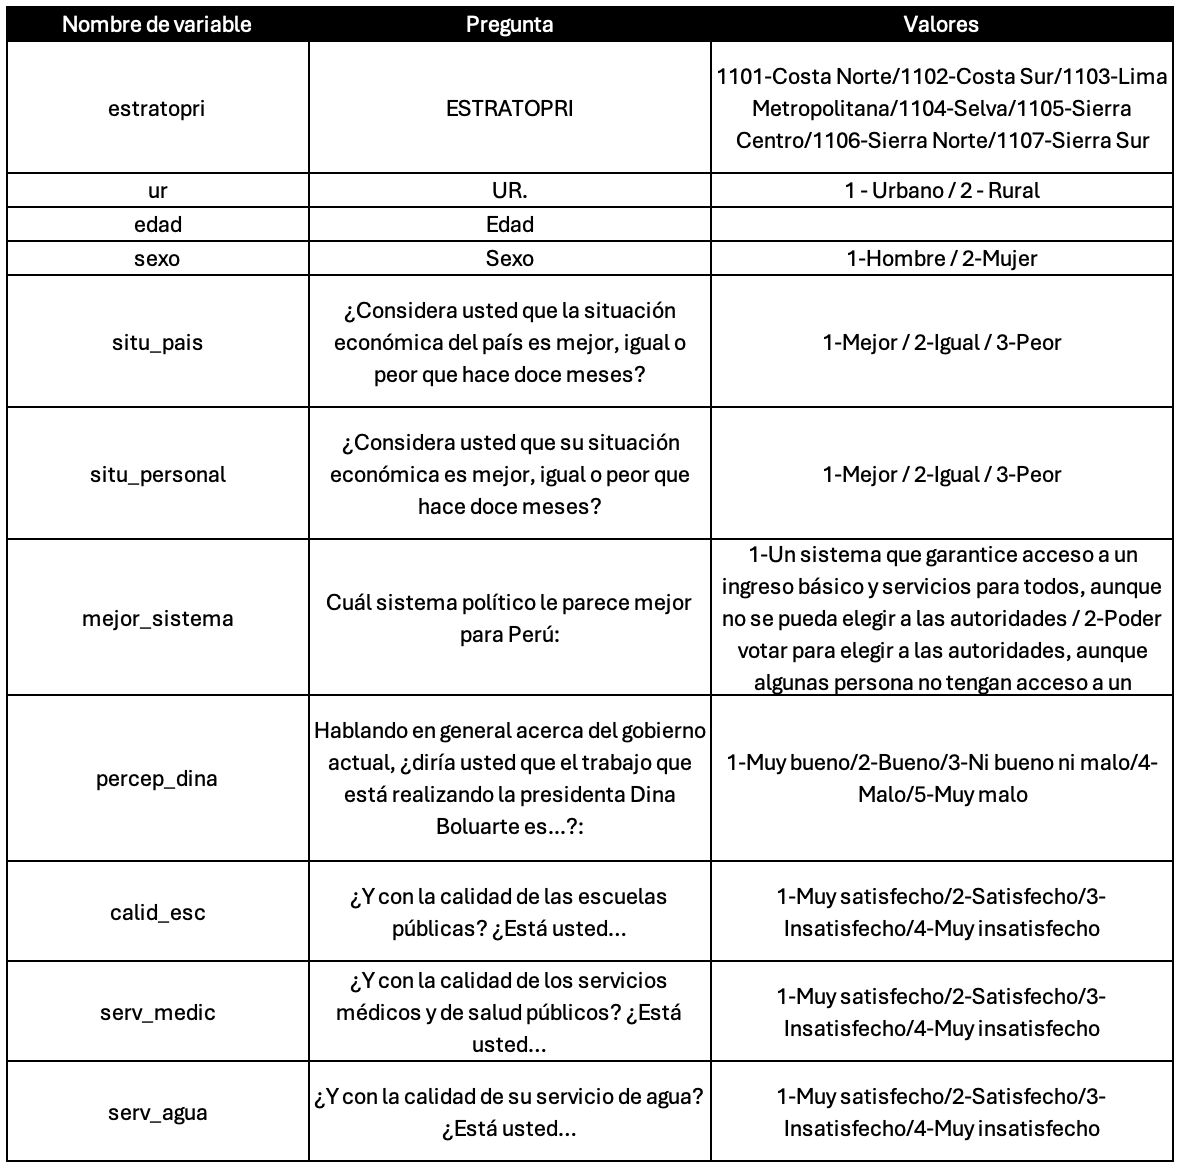
\includegraphics{diccionarioP7.jpeg}

¿Existe diferencia sobre la percepción económica actual entre hombres y
mujeres?

\begin{itemize}
\tightlist
\item
  Pregunta en cuestionario LAPOP: \emph{¿Considera usted que la
  situación económica del país es mejor, igual o peor que hace doce
  meses?}
\item
  Situación económica: 1 (Mejor), 2 (Igual), 3 (Peor)
\end{itemize}

\textbf{PASO 0: Revisamos la estructura de las variables que nos
interesan:}

\begin{Shaded}
\begin{Highlighting}[]
\NormalTok{lapop }\OtherTok{=}\NormalTok{ lapop }\SpecialCharTok{\%\textgreater{}\%}
  \FunctionTok{mutate}\NormalTok{(}\AttributeTok{situ\_pais =} \FunctionTok{factor}\NormalTok{(situ\_pais, }\AttributeTok{levels =} \DecValTok{1}\SpecialCharTok{:}\DecValTok{3}\NormalTok{, }\AttributeTok{labels =} \FunctionTok{c}\NormalTok{(}\StringTok{"Mejor"}\NormalTok{, }\StringTok{"Igual"}\NormalTok{, }\StringTok{"Peor"}\NormalTok{)))}

\FunctionTok{str}\NormalTok{(lapop}\SpecialCharTok{$}\NormalTok{situ\_pais) }\CommentTok{\#verificamos}
\end{Highlighting}
\end{Shaded}

\begin{verbatim}
##  Factor w/ 3 levels "Mejor","Igual",..: 3 3 2 1 3 3 3 3 3 3 ...
\end{verbatim}

A nivel general, ¿qué percibe la mayoría sobre la situación económica
del país?

\begin{Shaded}
\begin{Highlighting}[]
\NormalTok{resultados }\OtherTok{=}\NormalTok{ lapop }\SpecialCharTok{\%\textgreater{}\%}
  \FunctionTok{count}\NormalTok{(situ\_pais) }\SpecialCharTok{\%\textgreater{}\%}
  \FunctionTok{mutate}\NormalTok{(}\AttributeTok{porcentaje =} \FunctionTok{round}\NormalTok{(n }\SpecialCharTok{/} \FunctionTok{sum}\NormalTok{(n) }\SpecialCharTok{*} \DecValTok{100}\NormalTok{,}\DecValTok{2}\NormalTok{))}
\NormalTok{resultados}
\end{Highlighting}
\end{Shaded}

\begin{verbatim}
##   situ_pais   n porcentaje
## 1     Mejor  31       4.53
## 2     Igual 108      15.77
## 3      Peor 546      79.71
\end{verbatim}

Variable nominal sexo: 1 - Hombre / 2 - Mujer

\begin{Shaded}
\begin{Highlighting}[]
\FunctionTok{str}\NormalTok{(lapop}\SpecialCharTok{$}\NormalTok{sexo)}
\end{Highlighting}
\end{Shaded}

\begin{verbatim}
##  num [1:685] 2 2 1 1 1 1 2 2 2 1 ...
##  - attr(*, "format.spss")= chr "F8.2"
\end{verbatim}

\begin{Shaded}
\begin{Highlighting}[]
\FunctionTok{table}\NormalTok{(lapop}\SpecialCharTok{$}\NormalTok{sexo)}
\end{Highlighting}
\end{Shaded}

\begin{verbatim}
## 
##   1   2 
## 360 325
\end{verbatim}

Les damos el formato adecuado

\begin{Shaded}
\begin{Highlighting}[]
\NormalTok{lapop}\SpecialCharTok{$}\NormalTok{sexo }\OtherTok{=} \FunctionTok{factor}\NormalTok{(lapop}\SpecialCharTok{$}\NormalTok{sexo, }\AttributeTok{levels =} \DecValTok{1}\SpecialCharTok{:}\DecValTok{2}\NormalTok{, }\AttributeTok{labels =} \FunctionTok{c}\NormalTok{(}\StringTok{"Hombre"}\NormalTok{,}\StringTok{"Mujer"}\NormalTok{))}
\FunctionTok{table}\NormalTok{(lapop}\SpecialCharTok{$}\NormalTok{sexo)}
\end{Highlighting}
\end{Shaded}

\begin{verbatim}
## 
## Hombre  Mujer 
##    360    325
\end{verbatim}

\textbf{PASO 1: Tabla de contingencia}

Los valores observados son los valores de nuestra tabla tal como la
tenemos en nuestra base.

\begin{Shaded}
\begin{Highlighting}[]
\NormalTok{tabla1}\OtherTok{=}\FunctionTok{table}\NormalTok{(lapop}\SpecialCharTok{$}\NormalTok{situ\_pais, lapop}\SpecialCharTok{$}\NormalTok{sexo) }\CommentTok{\#tabla simple..luego se usará en la prueba chi}
\NormalTok{tabla1}
\end{Highlighting}
\end{Shaded}

\begin{verbatim}
##        
##         Hombre Mujer
##   Mejor     24     7
##   Igual     69    39
##   Peor     267   279
\end{verbatim}

\textbf{SUPUESTO}

Ten en cuenta que si te piden verificar el supuesto solo tienes que
solicitar la tabla de frecuencias esperadas y ver que efectivamente
todas las celdas tienen un número igual o mayor a 5.

\begin{Shaded}
\begin{Highlighting}[]
\FunctionTok{chisq.test}\NormalTok{(tabla1)}\SpecialCharTok{$}\NormalTok{expected}
\end{Highlighting}
\end{Shaded}

\begin{verbatim}
##        
##            Hombre     Mujer
##   Mejor  16.29197  14.70803
##   Igual  56.75912  51.24088
##   Peor  286.94891 259.05109
\end{verbatim}

En este caso sí cumple el supuesto!😎

Creamos porcentajes por columna, para ello tenemos que agregar
prop.table al comando anterior. El argumento de \texttt{prop.table}
puede ser

\begin{itemize}
\item
  1: \emph{para calcular porcentaje por \textbf{fila}}
\item
  2: \emph{para calcular por \textbf{columna}} ⚠️ Recuerda que es
  recomendable calcular los porcentajes sobre la variable
  sociodemográfica o aquella que antecede a la otra.
\end{itemize}

\begin{Shaded}
\begin{Highlighting}[]
\NormalTok{tablapor1 }\OtherTok{=}\NormalTok{ tabla1 }\SpecialCharTok{\%\textgreater{}\%}
           \FunctionTok{prop.table}\NormalTok{(}\DecValTok{2}\NormalTok{) }\SpecialCharTok{\%\textgreater{}\%}  
           \FunctionTok{round}\NormalTok{(}\DecValTok{2}\NormalTok{) }\CommentTok{\#redondear el resultado a 2 decimales}
\NormalTok{tablapor1}
\end{Highlighting}
\end{Shaded}

\begin{verbatim}
##        
##         Hombre Mujer
##   Mejor   0.07  0.02
##   Igual   0.19  0.12
##   Peor    0.74  0.86
\end{verbatim}

¿Existe diferencia con lo que vemos a nivel de cada subgrupo (hombre y
mujer) respecto a lo que habíamos visto a nivel de toda la muestra?

\textbf{PASO 2: Diagrama de barras apiladas}

\begin{Shaded}
\begin{Highlighting}[]
\NormalTok{toPlot1 }\OtherTok{=} \FunctionTok{as.data.frame}\NormalTok{(tablapor1) }
\FunctionTok{names}\NormalTok{(toPlot1) }\OtherTok{=} \FunctionTok{c}\NormalTok{(}\StringTok{"Categoria"}\NormalTok{, }\StringTok{"Sexo"}\NormalTok{, }\StringTok{"Porcentaje"}\NormalTok{)}
\end{Highlighting}
\end{Shaded}

Generamos el gráfico y lo solicitamos:

\begin{Shaded}
\begin{Highlighting}[]
\FunctionTok{library}\NormalTok{(ggplot2)}
\FunctionTok{library}\NormalTok{(ggsci) }\CommentTok{\#para usar la paleta de colores de startrek}

  \FunctionTok{ggplot}\NormalTok{(toPlot1, }\FunctionTok{aes}\NormalTok{(}\AttributeTok{x=}\NormalTok{Sexo, }\AttributeTok{y=}\NormalTok{Porcentaje}\SpecialCharTok{*}\DecValTok{100}\NormalTok{, }\AttributeTok{fill=}\NormalTok{Categoria)) }\SpecialCharTok{+}
  \FunctionTok{geom\_bar}\NormalTok{(}\AttributeTok{position=}\StringTok{"stack"}\NormalTok{, }\AttributeTok{stat=}\StringTok{"identity"}\NormalTok{)}\SpecialCharTok{+} \CommentTok{\#Stack indica que son barras apiladas}
  \FunctionTok{geom\_text}\NormalTok{(}\FunctionTok{aes}\NormalTok{(}\AttributeTok{label=}\FunctionTok{paste0}\NormalTok{(Porcentaje}\SpecialCharTok{*}\DecValTok{100}\NormalTok{,}\StringTok{"\%"}\NormalTok{)), }
            \AttributeTok{position =} \FunctionTok{position\_stack}\NormalTok{(}\AttributeTok{vjust =} \FloatTok{0.5}\NormalTok{), }
             \AttributeTok{size =} \DecValTok{4}\NormalTok{,}
             \AttributeTok{fontface=}\StringTok{"bold"}\NormalTok{)}\SpecialCharTok{+}
  \FunctionTok{labs}\NormalTok{(}\AttributeTok{x=}\StringTok{"Sexo"}\NormalTok{, }\AttributeTok{y=}\StringTok{"Porcentaje"}\NormalTok{, }\AttributeTok{fill=}\StringTok{"Situación económica"}\NormalTok{)}\SpecialCharTok{+}
    \FunctionTok{scale\_fill\_startrek}\NormalTok{()}\SpecialCharTok{+}
  \FunctionTok{theme\_minimal}\NormalTok{()}
\end{Highlighting}
\end{Shaded}

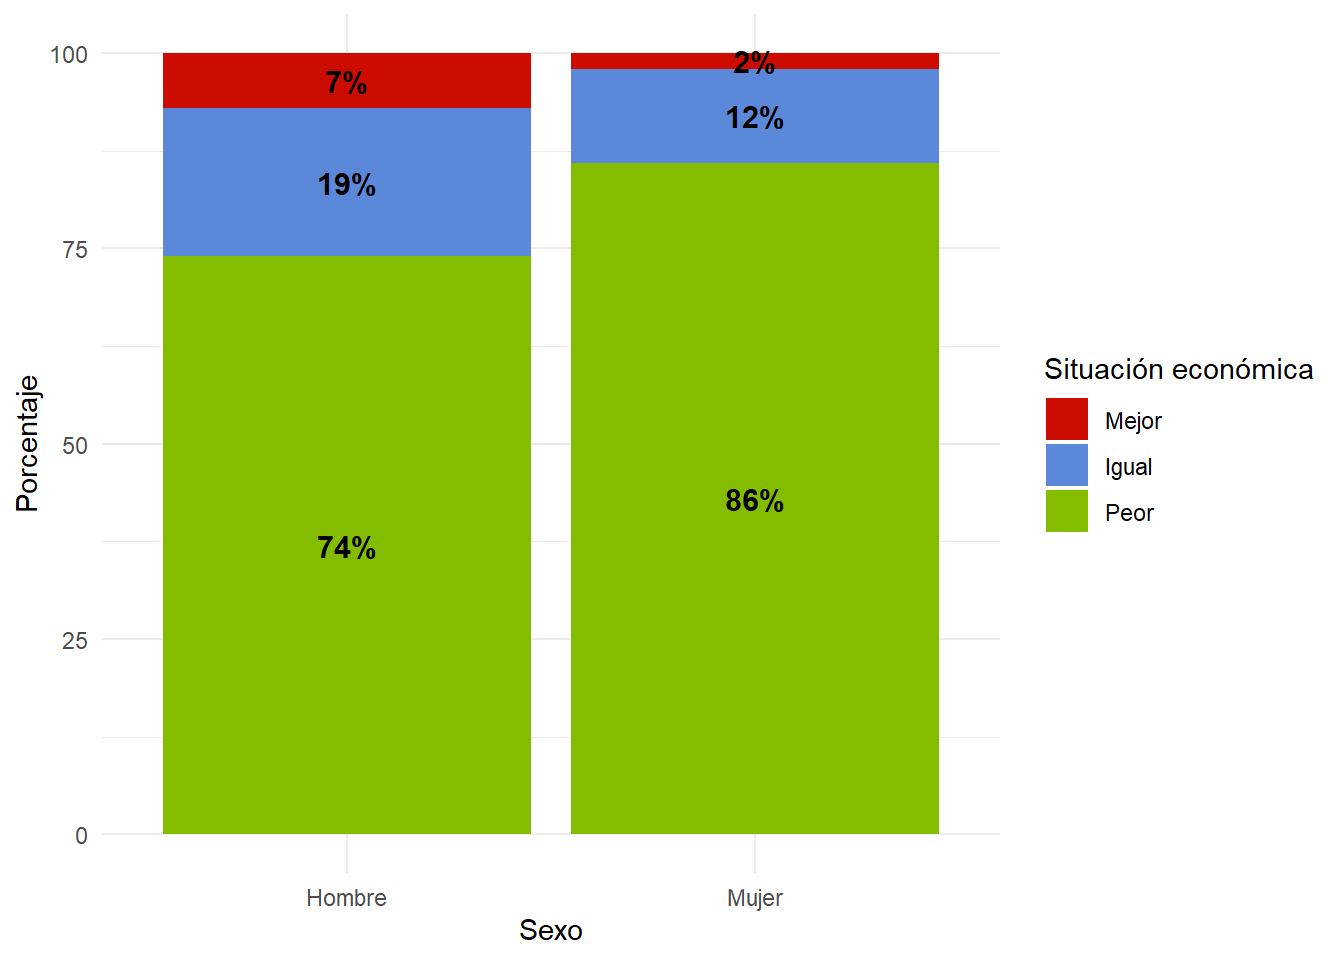
\includegraphics{semana6_practica_files/figure-latex/unnamed-chunk-10-1.pdf}

\begin{quote}
De forma preliminar ¿Hay diferencias entre la forma cómo se distribuye
la variable ``Situación Económica'' en cada subgrupo (hombre y mujer)?
\end{quote}

\textbf{PASO 3: Prueba Chi cuadrado}

\begin{itemize}
\item
  H0: El sexo es estadísticamente independiente de la situación
  económica respecto del año pasado
\item
  HA: El sexo es estadísticamente dependiente de la situación económica
  respecto del año pasado
\end{itemize}

Para hacer el test ingresamos la \textbf{tabla de frecuencias}

\begin{Shaded}
\begin{Highlighting}[]
\FunctionTok{chisq.test}\NormalTok{(tabla1)}
\end{Highlighting}
\end{Shaded}

\begin{verbatim}
## 
##  Pearson's Chi-squared test
## 
## data:  tabla1
## X-squared = 16.174, df = 2, p-value = 0.0003076
\end{verbatim}

De acuerdo al p-value obtenido en la prueba de hipótesis de Chi2, al ser
menor de 0.05, podemos rechazar la hipótesis nula (Las variables son
independientes).

Por lo tanto, concluimos existe dependencia entre las variables
escogidas: sexo y situación económica actual. Esto quiere decir que el
ser hombre o mujer \textbf{sí} se refleja en la percepción de la
situación económica del país.

¿Existe relación entre zona de vivienda y la percepción de la gestión de
Boluarte?

\emph{PASO 0: Revisamos la estructura de las variables que nos
interesan:}

\begin{itemize}
\tightlist
\item
  Variable percep\_dina: 1 (Muy bueno), 2 (Bueno), 3 (Ni bueno, ni
  malo), 4 (Malo), 5 (Muy malo).
\end{itemize}

Para este ejercicio creemos solo tres grupos ``Buena'' (1/Muy bueno y
2/Bueno), ``Ni buena ni mala'' (3/Ni bueno ni malo) y ``Mala'' (4/Malo,
5/Muy malo)

\begin{Shaded}
\begin{Highlighting}[]
\FunctionTok{str}\NormalTok{(lapop}\SpecialCharTok{$}\NormalTok{percep\_dina)}
\end{Highlighting}
\end{Shaded}

\begin{Shaded}
\begin{Highlighting}[]
\NormalTok{lapop }\OtherTok{=}\NormalTok{ lapop }\SpecialCharTok{\%\textgreater{}\%} 
  \FunctionTok{mutate}\NormalTok{(}\AttributeTok{percep\_dina2=}\FunctionTok{case\_when}\NormalTok{(percep\_dina}\SpecialCharTok{\textless{}=}\DecValTok{2} \SpecialCharTok{\textasciitilde{}} \StringTok{"Buena"}\NormalTok{,}
\NormalTok{                                percep\_dina}\SpecialCharTok{==}\DecValTok{3} \SpecialCharTok{\textasciitilde{}} \StringTok{"Ni buena ni mala"}\NormalTok{,}
\NormalTok{                                T }\SpecialCharTok{\textasciitilde{}} \StringTok{"Mala"}\NormalTok{))}

\NormalTok{lapop}\SpecialCharTok{$}\NormalTok{percep\_dina2 }\OtherTok{=} \FunctionTok{as.factor}\NormalTok{(lapop}\SpecialCharTok{$}\NormalTok{percep\_dina2)}
\end{Highlighting}
\end{Shaded}

Estrato: 1-Urbano/2-Rural

\begin{Shaded}
\begin{Highlighting}[]
\NormalTok{lapop}\SpecialCharTok{$}\NormalTok{ur }\OtherTok{=} \FunctionTok{factor}\NormalTok{(lapop}\SpecialCharTok{$}\NormalTok{ur, }
                      \AttributeTok{levels =} \FunctionTok{c}\NormalTok{(}\DecValTok{1}\SpecialCharTok{:}\DecValTok{2}\NormalTok{),}
                      \AttributeTok{labels =} \FunctionTok{c}\NormalTok{(}\StringTok{"Urbano"}\NormalTok{,}\StringTok{"Rural"}\NormalTok{))}
\FunctionTok{table}\NormalTok{(lapop}\SpecialCharTok{$}\NormalTok{ur)}
\end{Highlighting}
\end{Shaded}

\begin{verbatim}
## 
## Urbano  Rural 
##    536    149
\end{verbatim}

\textbf{PASO 1: Tabla de contingencia}

Los valores observados son los valores de nuestra tabla tal como la
tenemos en nuestra base

\begin{Shaded}
\begin{Highlighting}[]
\NormalTok{tabla2 }\OtherTok{=} \FunctionTok{table}\NormalTok{(lapop}\SpecialCharTok{$}\NormalTok{percep\_dina2, lapop}\SpecialCharTok{$}\NormalTok{ur)}
\NormalTok{tabla2}
\end{Highlighting}
\end{Shaded}

\begin{verbatim}
##                   
##                    Urbano Rural
##   Buena                39     5
##   Mala                292   106
##   Ni buena ni mala    205    38
\end{verbatim}

Es recomendable calcular los porcentajes sobre la variable
sociodemográfica o aquella que antecede a la otra. En este caso, esa
variable sería estrato (urbano/rural), por ello deberíamos calcular el
porcentaje sobre ella. Esto quiere decir que todas las percepciones
deben sumar 100\% para urbano y 100\% para rural.

\begin{Shaded}
\begin{Highlighting}[]
\NormalTok{tablapor2 }\OtherTok{=}\NormalTok{ tabla2 }\SpecialCharTok{\%\textgreater{}\%}
  \FunctionTok{prop.table}\NormalTok{(}\DecValTok{2}\NormalTok{) }\SpecialCharTok{\%\textgreater{}\%}  \CommentTok{\# porcentaje por columna, para calcular por fila indicar (1)}
  \FunctionTok{round}\NormalTok{(}\DecValTok{3}\NormalTok{)}
\NormalTok{tablapor2}
\end{Highlighting}
\end{Shaded}

\begin{verbatim}
##                   
##                    Urbano Rural
##   Buena             0.073 0.034
##   Mala              0.545 0.711
##   Ni buena ni mala  0.382 0.255
\end{verbatim}

\textbf{SUPUESTO}

Ten en cuenta que si te piden verificar el supuesto sólo tienes que
solicitar la tabla de frecuencias esperadas y ver que efectivamente
todas las celdas tienen un número igual o mayor a 5.

\begin{Shaded}
\begin{Highlighting}[]
\FunctionTok{chisq.test}\NormalTok{(tabla2)}\SpecialCharTok{$}\NormalTok{expected}
\end{Highlighting}
\end{Shaded}

\begin{verbatim}
##                   
##                      Urbano     Rural
##   Buena             34.4292  9.570803
##   Mala             311.4277 86.572263
##   Ni buena ni mala 190.1431 52.856934
\end{verbatim}

En este caso también cumple el supuesto!

\textbf{PASO 2: Diagrama de barras apiladas}

Preparamos la data para graficar:

\begin{Shaded}
\begin{Highlighting}[]
\NormalTok{toPlot2 }\OtherTok{=} \FunctionTok{as.data.frame}\NormalTok{(tablapor2) }
\FunctionTok{names}\NormalTok{(toPlot2) }\OtherTok{=} \FunctionTok{c}\NormalTok{(}\StringTok{"Categoria"}\NormalTok{, }\StringTok{"Estrato"}\NormalTok{, }\StringTok{"Porcentaje"}\NormalTok{)}
\end{Highlighting}
\end{Shaded}

Generamos el gráfico y lo solicitamos:

\begin{Shaded}
\begin{Highlighting}[]
\FunctionTok{library}\NormalTok{(tayloRswift)}
  \FunctionTok{ggplot}\NormalTok{(toPlot2, }\FunctionTok{aes}\NormalTok{(}\AttributeTok{x=}\NormalTok{Estrato, }\AttributeTok{y=}\NormalTok{Porcentaje}\SpecialCharTok{*}\DecValTok{100}\NormalTok{, }\AttributeTok{fill=}\NormalTok{Categoria)) }\SpecialCharTok{+}
  \FunctionTok{geom\_bar}\NormalTok{(}\AttributeTok{position=}\StringTok{"stack"}\NormalTok{, }\AttributeTok{stat=}\StringTok{"identity"}\NormalTok{)}\SpecialCharTok{+}
  \FunctionTok{geom\_text}\NormalTok{(}\FunctionTok{aes}\NormalTok{(}\AttributeTok{label=}\FunctionTok{paste}\NormalTok{(Porcentaje}\SpecialCharTok{*}\DecValTok{100}\NormalTok{,}\StringTok{"\%"}\NormalTok{)), }
            \AttributeTok{position =} \FunctionTok{position\_stack}\NormalTok{(}\AttributeTok{vjust=}\FloatTok{0.5}\NormalTok{), }
             \AttributeTok{size =} \DecValTok{3}\NormalTok{, }\AttributeTok{fontface=}\StringTok{"bold"}\NormalTok{)}\SpecialCharTok{+}
  \FunctionTok{labs}\NormalTok{(}\AttributeTok{x=}\StringTok{"Estrato"}\NormalTok{, }\AttributeTok{y=}\StringTok{"Categoría"}\NormalTok{, }\AttributeTok{fill=}\StringTok{"Confianza"}\NormalTok{)}\SpecialCharTok{+}
    \FunctionTok{scale\_fill\_taylor}\NormalTok{(}\AttributeTok{palette=}\StringTok{"lover"}\NormalTok{)}\SpecialCharTok{+}
  \FunctionTok{theme\_bw}\NormalTok{()}
\end{Highlighting}
\end{Shaded}

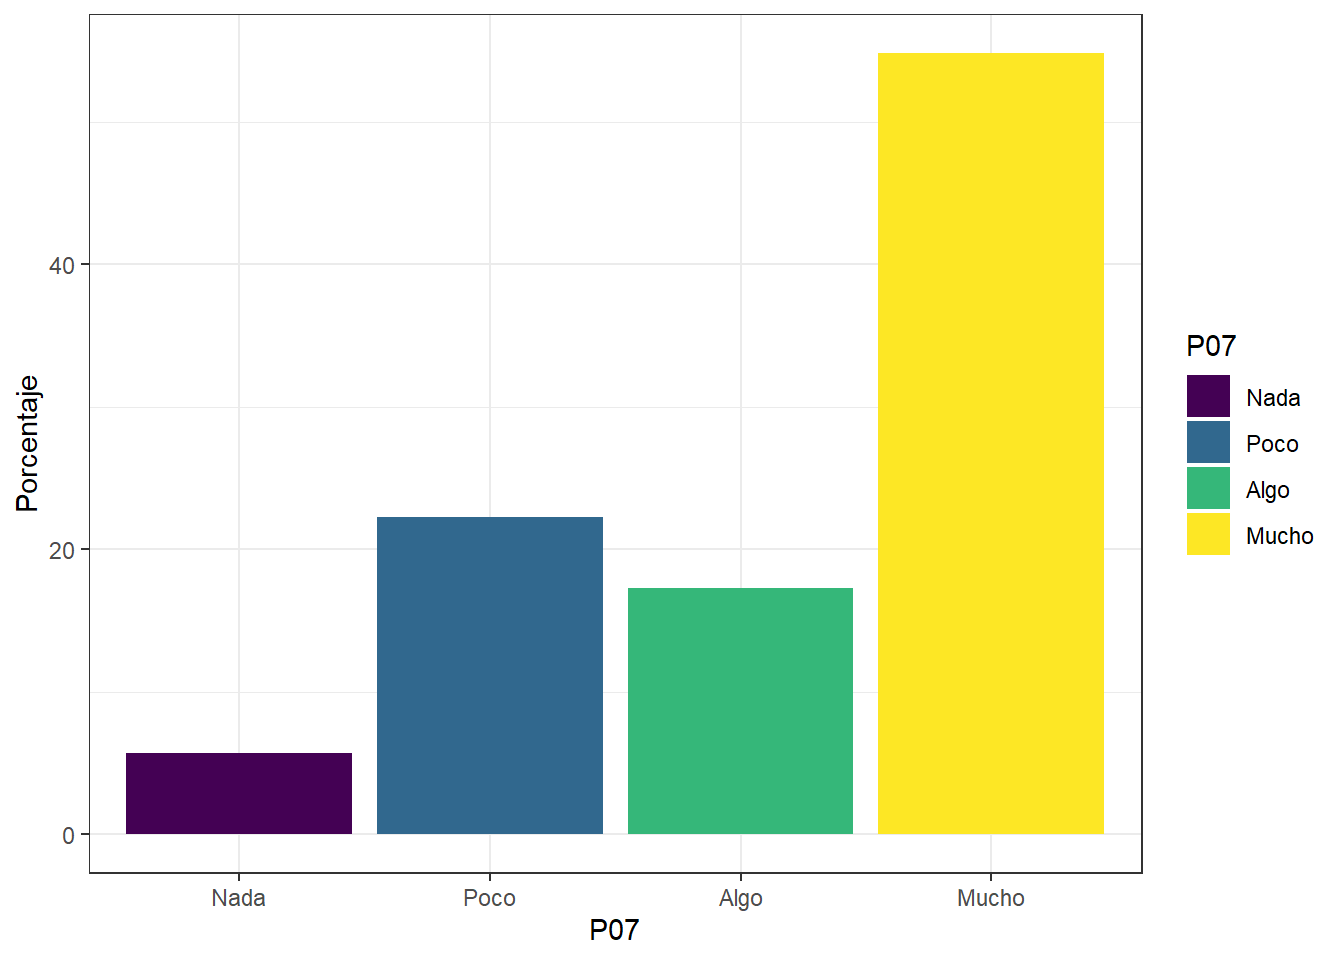
\includegraphics{semana6_practica_files/figure-latex/unnamed-chunk-19-1.pdf}

\textbf{PASO 3: Prueba Chi cuadrado}

\begin{itemize}
\item
  H0: La percepción de la gestión de Dina es estadísticamente
  independiente del estrato del encuestado
\item
  HA: La percepción de la gestión de Dina es estadísticamente
  dependiente del estrato del encuestado
\end{itemize}

\begin{Shaded}
\begin{Highlighting}[]
\FunctionTok{chisq.test}\NormalTok{(tabla2)}
\end{Highlighting}
\end{Shaded}

\begin{verbatim}
## 
##  Pearson's Chi-squared test
## 
## data:  tabla2
## X-squared = 13.698, df = 2, p-value = 0.00106
\end{verbatim}

🗯️ De acuerdo al p-value obtenido en la prueba de hipótesis de Chi2, al
ser menor de 0.05, podemos rechazar la hipótesis nula (Las variables son
independientes).

Por lo tanto, concluimos que la variable percepción de la gestión de
Dina y el estrato de residencia sí se encuentran asociadas. Una mayor
proporción de los residentes de las zonas rurales califican como mala a
la gestión de la presidenta; mientras que, la zona urbana se relaciona
con una mayor proporción de opiniones neutrales en comparación.

\hypertarget{ejercicios-en-clase}{%
\subsection{Ejercicios en clase:}\label{ejercicios-en-clase}}

1. Analizar si existe asociación entre las variables satisfacción con la
de situación de las escuelas (calid\_esc) y edad (agrupado)\\
Para ello debes agrupar edad, de tal manera que las categorías sean:

\begin{itemize}
\item
  De 18 a 25
\item
  De 26 a 40
\item
  De 40 a 60
\item
  Más de 60
\end{itemize}

\emph{Hint}: Usa case\_when y establece los intervalos, no olvides que
la estructura es case\_when(condición \textasciitilde{} valor,
condicion2 \textasciitilde{} valor2,\ldots)

\begin{enumerate}
\def\labelenumi{\arabic{enumi}.}
\setcounter{enumi}{1}
\tightlist
\item
  Analizar si existe dependencia entre la variable estrato y
  satisfacción con la situación de servicios médicos (serv\_medic)
\end{enumerate}

\hypertarget{ejercicios-para-casa}{%
\subsection{Ejercicios para casa:}\label{ejercicios-para-casa}}

\begin{enumerate}
\def\labelenumi{\arabic{enumi}.}
\item
  Analizar la asociación entre la región (estratropri) (Agrupar y
  obtener Costa/Sierra/Selva/Lima Metropolitana) y la satisfacción con
  la calidad del servicio de agua (serv\_agua).

  1101/1102 - Costa

  1103 - Lima Metropolitana

  1104 - Selva

  1105/1106/1107 - Sierra
\item
  Crea un indice aditivo de la satisfacción con servicios públicos que
  vaya del 0 al 10. Previamente, debes invertir el sentido de las
  variables: calid\_esc, serv\_medic y serv\_agua. Lo que era 4, ahora
  debe ser 1, lo que era 3 ahora 2, lo que era 2 ahora 3 y lo que era 1
  ahora 4. Así, lo que se convierta en 4 medida la satisfacción y no la
  insatisfacción. Luego de ello, lo que supere el valor de en el
  indicador será ``Satisfecho con servicios públicos'' o 5 o menos será
  ``Insatisfecho con los servicios públicos'', esta nueva variable será
  llamada ind\_agrupado. Analiza si ind\_agrupado se encuentra asociado
  con el sexo del encuestado.
\end{enumerate}

\end{document}
